\documentclass[aspectratio=169,10pt]{beamer}

\usepackage[T1]{fontenc}
\usepackage{lmodern}
\usepackage{microtype}
\usepackage{booktabs}
\usepackage{tabularx}
\newcolumntype{P}[1]{>{\raggedright\arraybackslash}p{#1}}
\newcolumntype{Y}{>{\raggedright\arraybackslash}X}
\usepackage{tikz}
\usepackage{listings}
\usepackage{amsmath}
\usepackage{hyperref}
\usetikzlibrary{arrows.meta,positioning,calc,fit,shapes.geometric}

% Visual system adapted from the supplied QueryForge reference deck.
% The reference deck uses one dominant indigo, a white canvas, black body copy,
% compact blue markers, and page numbers at the lower-right corner.
\definecolor{QFNavy}{HTML}{171717}
\definecolor{QFBlue}{HTML}{3737B8}
\definecolor{QFCyan}{HTML}{0891B2}
\definecolor{QFTeal}{HTML}{0F766E}
\definecolor{QFGreen}{HTML}{16A34A}
\definecolor{QFOrange}{HTML}{EA580C}
\definecolor{QFRed}{HTML}{DC2626}
\definecolor{QFSlate}{HTML}{475467}
\definecolor{QFLight}{HTML}{F4F7FB}
\definecolor{QFLine}{HTML}{D0D5DD}

\setbeamercolor{normal text}{fg=black,bg=white}
\setbeamercolor{structure}{fg=QFBlue}
\setbeamercolor{frametitle}{fg=white,bg=QFBlue}
\setbeamercolor{alerted text}{fg=QFOrange}
\setbeamerfont{frametitle}{size=\fontsize{17}{20}\selectfont,series=\mdseries}
\setbeamerfont{title}{size=\fontsize{18}{23}\selectfont,series=\mdseries}
\setbeamerfont{subtitle}{size=\large}
\setbeamertemplate{navigation symbols}{}
\setbeamertemplate{itemize item}{\color{QFBlue}\raise0.18ex\hbox{\scriptsize$\bullet$}}
\setbeamertemplate{itemize subitem}{\color{QFBlue}\raise0.12ex\hbox{\tiny$\bullet$}}
\setbeamercolor{enumerate item}{fg=QFBlue}
\setbeamercolor{enumerate subitem}{fg=QFBlue}
\setbeamertemplate{frametitle}{%
  \nointerlineskip
  \begin{beamercolorbox}[wd=\paperwidth,ht=.72cm,dp=.20cm,leftskip=.27cm]{frametitle}%
    \insertframetitle
  \end{beamercolorbox}}
\setbeamertemplate{footline}{%
  \hfill\raisebox{.13cm}{\scriptsize\insertframenumber\,/\,\inserttotalframenumber\hspace{.22cm}}}

\newcommand{\metric}[3]{%
  \begin{tikzpicture}[baseline]
    \node[rounded corners=5pt,fill=#1!9,draw=#1!35,minimum width=2.35cm,
      minimum height=1.05cm,align=center,inner sep=5pt]
      {\color{#1}\bfseries\large #2\\[-1pt]\color{QFSlate}\scriptsize #3};
  \end{tikzpicture}}
\newcommand{\pill}[2]{\tikz[baseline=(x.base)]\node[rounded corners=4pt,fill=#1!10,
  text=#1,inner xsep=6pt,inner ysep=3pt,font=\scriptsize\bfseries](x){#2};}
\newcommand{\evidence}{\scriptsize\color{QFSlate}Source: repository tests and deployment checks, 23 October 2026.}

\lstset{basicstyle=\ttfamily\scriptsize,keywordstyle=\color{QFBlue}\bfseries,
  commentstyle=\color{QFSlate},stringstyle=\color{QFTeal},showstringspaces=false,
  frame=single,rulecolor=\color{QFLine},backgroundcolor=\color{QFLight},
  breaklines=true,columns=fullflexible}


\newcommand{\items}{\setlength\itemsep{.20cm}}
\title{Relief Desk: Real-Time Disaster Emergency\\and Relief Coordination}
\subtitle{Cloud Computing Course Project}
% Edit the author field to add the complete project team and roll numbers.
\author{}
\institute{Cloud Computing Course Project}
\date{October 23, 2026}
\begin{document}
\begin{frame}[plain]
  \begin{tikzpicture}[remember picture,overlay]
    \node[rounded corners=5pt,fill=black!28,minimum width=.97\paperwidth,
      minimum height=1.55cm] at ([xshift=.06cm,yshift=1.28cm]current page.center) {};
    \node[rounded corners=5pt,fill=QFBlue,text=white,minimum width=.97\paperwidth,
      minimum height=1.55cm,align=center,text width=.90\paperwidth]
      at ([yshift=1.35cm]current page.center)
      {\usebeamerfont{title}\inserttitle};
    \node[align=center] at ([yshift=-.65cm]current page.center)
      {\insertauthor\;---\;\insertinstitute\\[2pt]\insertdate};
    \node[anchor=south east,font=\scriptsize] at ([xshift=-.22cm,yshift=.13cm]current page.south east)
      {\insertframenumber\,/\,\inserttotalframenumber};
  \end{tikzpicture}
\end{frame}

% 2: Problem statement
\begin{frame}{Problem statement: coordination fragments during a disaster}
\begin{columns}[T,onlytextwidth]
\column{.52\textwidth}
\textbf{Reports, teams, and supplies must stay consistent while many people act at once.}
\vspace{.20cm}
\begin{itemize}\items
\item Incident details can be scattered across calls, messages, and spreadsheets.
\item Responders may work from stale information.
\item Competing requests can promise the same supplies twice.
\item Critical reports and overdue requests need follow-up.
\item Evidence and responsibility need a shared record.
\end{itemize}
\column{.44\textwidth}
\centering
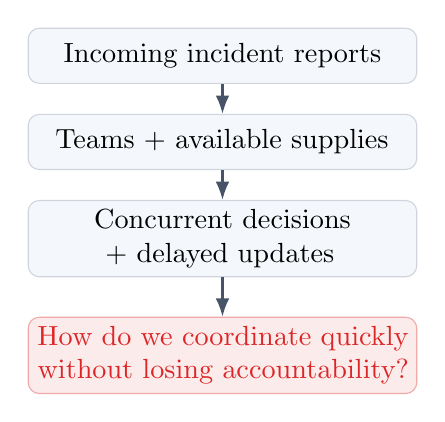
\begin{tikzpicture}[node distance=.38cm,
 b/.style={rounded corners,draw=QFLine,fill=QFLight,text width=4.7cm,minimum height=.7cm,align=center},a/.style={-{Latex},thick,QFSlate}]
\node[b](r){Incoming incident reports};
\node[b,below=of r](t){Teams + available supplies};
\node[b,below=of t](c){Concurrent decisions + delayed updates};
\node[b,below=.5cm of c,fill=QFRed!9,draw=QFRed!40,text=QFRed](q){How do we coordinate quickly\\without losing accountability?};
\draw[a](r)--(t);\draw[a](t)--(c);\draw[a](c)--(q);
\end{tikzpicture}
\end{columns}
\end{frame}

% 3: Existing approaches
\begin{frame}{Existing approaches---and the course project gap}
\small
\begin{tabularx}{\textwidth}{@{}P{2.7cm}P{3.6cm}Y@{}}
\toprule
\textbf{Approach} & \textbf{Useful capability} & \textbf{What this project brings together}\\\midrule
Calls and group messaging & Fast communication between people & Structured incident status, ownership, and an activity history\\\addlinespace[.2cm]
Shared spreadsheets & Simple lists of teams and supplies & Server-side permissions and atomic dispatch validation\\\addlinespace[.2cm]
Generic task boards & Assignment and task progress & Linked incidents, relief requests, inventory, and evidence files\\\addlinespace[.2cm]
Separate cloud services & Managed storage, compute, and messaging & One working application showing how the services cooperate\\\bottomrule
\end{tabularx}\par
\vspace{.4cm}
\textbf{Project objective:} demonstrate a secure, event-driven coordination workflow using managed cloud services.
\vspace{.2cm}

{\scriptsize\color{QFSlate}Design comparison of common workflow patterns; not a benchmark of commercial disaster-management products.}
\end{frame}

% 4: Service mapping
\begin{frame}{Our solution: one workspace, seven cloud capabilities}
\small
\begin{tabularx}{\textwidth}{@{}P{3.1cm}P{3.5cm}Y@{}}
\toprule
\textbf{Cloud service} & \textbf{Responsibility} & \textbf{Visible application behavior}\\\midrule
Cloudflare Workers & Serverless application and API & Dashboard, validation, permissions, business actions\\\addlinespace
Cloudflare D1 & Relational persistence & Incidents, members, teams, stock, requests, activity\\\addlinespace
Cloudflare Access & Identity and access boundary & Allowlisted member sign-in and verified identity\\\addlinespace
Cloudflare R2 & Private object storage & Incident photos and PDF attachments\\\addlinespace
Cloudflare Queues & Asynchronous processing & Critical-incident and dispatch notifications\\\addlinespace
Cron Triggers & Scheduled background work & Five-minute escalation and low-stock checks\\\addlinespace
Durable Objects & Stateful WebSocket rooms & Live updates, workspace presence, incident viewers\\\bottomrule
\end{tabularx}\par
\vspace{.25cm}
\pill{QFBlue}{MANAGED COMPUTE}\quad\pill{QFTeal}{DURABLE DATA}\quad\pill{QFOrange}{EVENT-DRIVEN WORK}
\end{frame}

% 5: Architecture
\begin{frame}{System architecture}
\centering
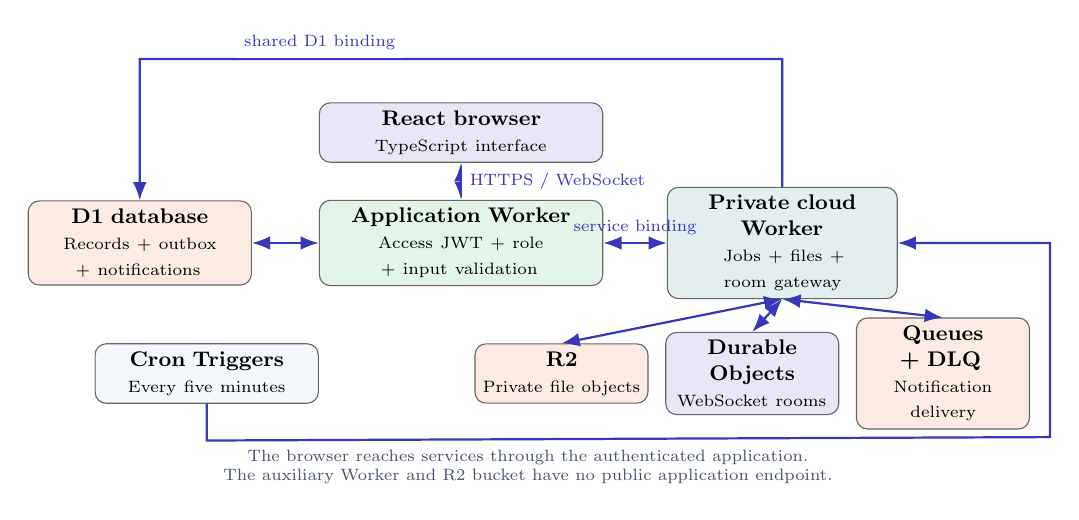
\begin{tikzpicture}[scale=.85,transform shape,
 b/.style={rounded corners=4pt,draw=black!60,align=center,minimum height=.72cm,font=\small},
 a/.style={-{Latex},thick,QFBlue},bi/.style={{Latex}-{Latex},thick,QFBlue}]
\node[b,fill=QFBlue!12,text width=4cm](ui) at (0,2.6){\textbf{React browser}\\\scriptsize TypeScript interface};
\node[b,fill=QFGreen!12,text width=4cm](app) at (0,.95){\textbf{Application Worker}\\\scriptsize Access JWT + role + input validation};
\node[b,fill=QFOrange!12,text width=3.1cm](db) at (-4.8,.95){\textbf{D1 database}\\\scriptsize Records + outbox + notifications};
\node[b,fill=QFTeal!12,text width=3.2cm](svc) at (4.8,.95){\textbf{Private cloud Worker}\\\scriptsize Jobs + files + room gateway};
\node[b,fill=QFOrange!12,text width=2.35cm](r2) at (1.5,-1.0){\textbf{R2}\\\scriptsize Private file objects};
\node[b,fill=QFBlue!12,text width=2.35cm](do) at (4.35,-1.0){\textbf{Durable Objects}\\\scriptsize WebSocket rooms};
\node[b,fill=QFOrange!12,text width=2.35cm](queue) at (7.2,-1.0){\textbf{Queues + DLQ}\\\scriptsize Notification delivery};
\node[b,fill=QFLight,text width=3.1cm](cron) at (-3.8,-1.0){\textbf{Cron Triggers}\\\scriptsize Every five minutes};
\draw[bi](ui)--node[right,font=\scriptsize,fill=white]{HTTPS / WebSocket}(app);
\draw[bi](app)--(db);
\draw[bi](app)--node[above,font=\scriptsize]{service binding}(svc);
\draw[a](svc.north)--(4.8,3.7)--node[pos=.72,above,font=\scriptsize,fill=white]{shared D1 binding}(-4.8,3.7)--(db.north);
\draw[bi](svc.south)--(do.north);
\draw[bi](svc.south)--(r2.north);
\draw[bi](svc.south)--(queue.north);
\draw[a](cron.south)--++(0,-.55)--(8.8,-1.95)--(8.8,.95)--(svc.east);
\node[font=\scriptsize,text=QFSlate,align=center] at (1,-2.4){The browser reaches services through the authenticated application.\\The auxiliary Worker and R2 bucket have no public application endpoint.};
\end{tikzpicture}
\end{frame}

% 6: Workflow
\begin{frame}{What happens after a user reports an incident?}
\centering
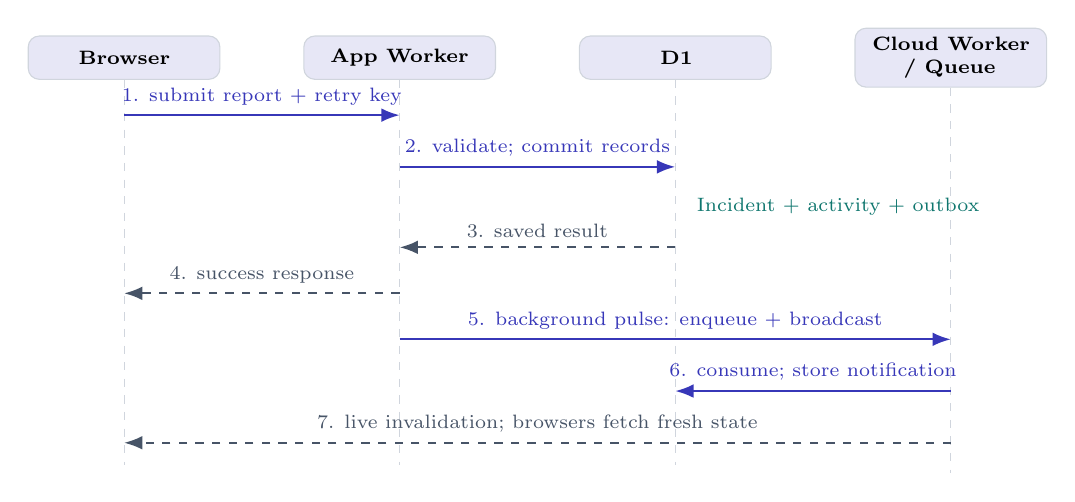
\begin{tikzpicture}[x=1cm,y=.73cm,
 actor/.style={rounded corners,fill=QFBlue!12,draw=QFLine,text width=2.2cm,minimum height=.55cm,align=center,font=\scriptsize\bfseries},
 a/.style={-{Latex},thick,QFBlue},r/.style={-{Latex},dashed,thick,QFSlate}]
\node[actor](u)at(0,2.8){Browser};\node[actor](w)at(3.5,2.8){App Worker};
\node[actor](d)at(7,2.8){D1};\node[actor](c)at(10.5,2.8){Cloud Worker / Queue};
\foreach \n in {u,w,d,c}\draw[dashed,QFLine](\n.south)--++(0,-6.7);
\draw[a](0,1.8)--node[above,font=\scriptsize]{1. submit report + retry key}(3.5,1.8);
\draw[a](3.5,.9)--node[above,font=\scriptsize]{2. validate; commit records}(7,.9);
\node[font=\scriptsize,align=left,anchor=west,text=QFTeal] at(7.15,.2){Incident + activity + outbox};
\draw[r](7,-.5)--node[above,font=\scriptsize]{3. saved result}(3.5,-.5);
\draw[r](3.5,-1.3)--node[above,font=\scriptsize]{4. success response}(0,-1.3);
\draw[a](3.5,-2.1)--node[above,font=\scriptsize]{5. background pulse: enqueue + broadcast}(10.5,-2.1);
\draw[a](10.5,-3)--node[above,font=\scriptsize]{6. consume; store notification}(7,-3);
\draw[r](10.5,-3.9)--node[above,font=\scriptsize]{7. live invalidation; browsers fetch fresh state}(0,-3.9);
\end{tikzpicture}
\vspace{.12cm}

\scriptsize\textbf{Key separation:} the report is saved before asynchronous notification processing completes.
\end{frame}

% 7: Users
\begin{frame}{User workflow and role-based access}
\footnotesize
\begin{tabularx}{\textwidth}{@{}P{3.7cm}YYY@{}}
\toprule
\textbf{Capability}&\textbf{Reporter}&\textbf{Responder}&\textbf{Coordinator}\\\midrule
View workspace & Yes & Yes & Yes\\
Report / request & Yes & Yes & Yes\\
Upload evidence & Yes & Yes & Yes\\
Assign / dispatch & --- & Yes & Yes\\
Acknowledge alerts & --- & Yes & Yes\\
Manage stock / teams & --- & --- & Yes\\
Manage roles / run checks & --- & --- & Yes\\\bottomrule
\end{tabularx}\par
\vspace{.3cm}
\textbf{Typical sequence}\par\vspace{.1cm}
Sign in $\rightarrow$ report $\rightarrow$ attach evidence $\rightarrow$ assign team $\rightarrow$ request supplies $\rightarrow$ dispatch $\rightarrow$ resolve.
\vspace{.25cm}

{\scriptsize\color{QFSlate}Access policy controls who can enter; application roles control what they can do. New members join as reporters after the initial coordinator is established. File deletion is limited to its uploader or a coordinator.}
\end{frame}

% 8: Inventory integrity
\begin{frame}{Supply dispatch: correctness under concurrent requests}
\begin{columns}[T,onlytextwidth]
\column{.52\textwidth}
\textbf{D1 is the authority for stock changes.}
\begin{itemize}\items
\item Validate role, request state, and record version.
\item SQL triggers reject insufficient inventory.
\item Stock deduction and dispatch status commit together.
\item Idempotency receipts make repeated action retries safe.
\item Pending requests block incident resolution.
\end{itemize}
\column{.44\textwidth}
\centering
\metric{QFBlue}{100 kits}{illustrative starting inventory}
\vspace{.22cm}

\metric{QFTeal}{20 kits}{one successful dispatch}
\vspace{.22cm}

\metric{QFGreen}{80 kits}{stock after dispatch and retry}
\vspace{.2cm}

{\scriptsize\color{QFSlate}Example workflow, not a performance measurement. A second independent request must still pass the available-stock check.}
\end{columns}
\end{frame}

% 9: R2
\begin{frame}{Incident evidence: private files with controlled access}
\begin{columns}[T,onlytextwidth]
\column{.53\textwidth}
\textbf{R2 stores bytes; D1 stores ownership and metadata.}
\begin{enumerate}\items
\item Authenticate the uploader and validate the incident.
\item Check file size, allowed type, and file signature.
\item Reserve metadata with an uploading state.
\item Store the object in the private R2 bucket.
\item Mark ready and append an activity entry.
\end{enumerate}
\vspace{.15cm}
Downloads pass through the app's identity boundary. Interrupted transfers are reconciled by scheduled cleanup after one hour.
\column{.43\textwidth}
\centering
\metric{QFBlue}{5 MB}{maximum per file}\quad
\metric{QFTeal}{20 files}{maximum per incident}
\vspace{.22cm}

\metric{QFOrange}{500 MB}{workspace attachment cap}
\vspace{.25cm}

\pill{QFBlue}{JPG}\quad\pill{QFBlue}{PNG}\quad\pill{QFBlue}{PDF}
\vspace{.25cm}

{\scriptsize\color{QFSlate}File signature checks are basic type validation; malware scanning is not implemented.}
\end{columns}
\end{frame}

% 10: Queue + cron
\begin{frame}{Queued notifications and scheduled escalation checks}
\begin{columns}[T,onlytextwidth]
\column{.49\textwidth}
\textbf{Event-driven notifications}
\begin{itemize}\items
\item Critical report and supply dispatch events create in-app alerts.
\item The activity transaction also inserts an outbox record.
\item Queues decouples processing from the user request.
\item Stable notification IDs prevent duplicate rows on redelivery.
\item Failed deliveries retry; a dead-letter queue is configured.
\end{itemize}
\column{.47\textwidth}
\textbf{Cron: every five minutes}
\vspace{.15cm}

\small
\begin{tabularx}{\linewidth}{@{}Yr@{}}\toprule
\textbf{Condition}&\textbf{Threshold}\\\midrule
Critical incident unassigned & 30 min\\\addlinespace
Relief request pending & 60 min\\\addlinespace
Supply quantity low & $\leq 10$ units\\\bottomrule
\end{tabularx}\par
\vspace{.25cm}
\begin{itemize}\items
\item Coordinator: \textbf{Check now} runs the same checks.
\item Responder/coordinator: acknowledge an alert.
\item Acknowledgment does not resolve its underlying condition.
\end{itemize}
\end{columns}
\vspace{.16cm}
{\scriptsize\color{QFSlate}Queues uses at-least-once delivery [1]. Application processing is idempotent; alerts are not email or SMS.}
\end{frame}

% 11: Real-time + recovery
\begin{frame}{Real-time coordination with explicit recovery paths}
\begin{columns}[T,onlytextwidth]
\column{.49\textwidth}
\textbf{Durable Object rooms}
\begin{itemize}\items
\item Workspace room broadcasts change notifications and presence.
\item Incident rooms show who is viewing the same report.
\item WebSocket hibernation keeps idle connections available [2].
\item Connections renew authentication after approximately five minutes.
\item Hidden tabs pause connections; visible tabs reconnect.
\end{itemize}
\column{.47\textwidth}
\textbf{Failure $\rightarrow$ recovery}
\small
\begin{tabularx}{\linewidth}{@{}P{2cm}Y@{}}\toprule
\textbf{Failure}&\textbf{Recovery mechanism}\\\midrule
Connection lost & Reconnect with backoff; refresh state\\\addlinespace
Missed broadcast & 30-second snapshot fallback\\\addlinespace
Queue send fails & Persisted outbox retried by scans\\\addlinespace
Duplicate delivery & Idempotent notification insertion\\\addlinespace
Stale user edit & Version conflict; refresh and retry\\\bottomrule
\end{tabularx}
\end{columns}
\vspace{.25cm}
\pill{QFBlue}{D1: BUSINESS STATE}\quad\pill{QFTeal}{WEBSOCKETS: CHANGE SIGNALS}
\end{frame}

% 12: Evaluation
\begin{frame}{Evaluation: tested behavior and deployment evidence}
\begin{columns}[T,onlytextwidth]
\column{.55\textwidth}
\textbf{What the automated checks cover}
\begin{itemize}\items
\item Stock concurrency, duplicate dispatch, stale edits, and rollback.
\item Access JWT validation, roles, cross-origin rejection, and file ownership.
\item Queue duplicates and retries; scheduled alert conditions.
\item Upload validation, download, deletion, and retry behavior.
\item Two-browser live updates, reconnects, and mobile layout.
\end{itemize}
\column{.41\textwidth}
\centering
\metric{QFBlue}{17 passed}{database / security tests}
\vspace{.18cm}

\metric{QFTeal}{7 passed}{browser workflow tests}
\vspace{.18cm}

\pill{QFGreen}{TYPE CHECK: PASS}\quad\pill{QFGreen}{BUILD: PASS}
\vspace{.2cm}

\evidence
\end{columns}
\vspace{.18cm}
{\scriptsize\color{QFSlate}Both Workers and cloud bindings were deployed. Access redirects and production WebSocket traffic were observed. These test counts are local verification, not a production load test or availability guarantee. First automatic Cron execution was not observed in the recorded deployment check.}
\end{frame}

% 13: Challenges
\begin{frame}{Engineering challenges---and how we addressed them}
\small
\begin{tabularx}{\textwidth}{@{}P{2.6cm}P{4cm}Y@{}}\toprule
\textbf{Challenge}&\textbf{Failure mode}&\textbf{Resolution}\\\midrule
Concurrent dispatch & Two responders consume the same stock & Atomic D1 transaction and stock guards\\\addlinespace[.16cm]
Retry after timeout & A successful action is submitted again & Mutation receipts and version checks\\\addlinespace[.16cm]
Database / queue boundary & Saved event never reaches the queue & Transactional outbox plus scheduled retries\\\addlinespace[.16cm]
File / metadata boundary & Upload or deletion stops halfway & Explicit file states and delayed cleanup\\\addlinespace[.16cm]
WebSocket authentication & Local upgrades bypass HTTP middleware & Development-only identity handling; production Access verification\\\addlinespace[.16cm]
Member onboarding & Email-domain rule used for one address & Exact-email allow rule and enabled one-time PIN login\\\bottomrule
\end{tabularx}\par
\vspace{.25cm}
\textbf{Lesson:} define the durable state and authorization boundary before adding retries or live updates.
\end{frame}

% 14: Boundaries
\begin{frame}{Limitations and future work}
\begin{columns}[T,onlytextwidth]
\column{.49\textwidth}
\textbf{Current boundaries}
\begin{itemize}\items
\item Course demonstration; not connected to emergency services.
\item Reports are user-entered; no verified disaster-data feed.
\item Alerts are in-app; no email, SMS, or push delivery.
\item Scheduled checks are periodic, not hard real-time deadlines.
\item Included cloud quotas and application storage caps are finite.
\item No production-scale load, disaster-recovery, or availability study.
\end{itemize}
\column{.47\textwidth}
\textbf{Next milestones}
\begin{enumerate}\items
\item Integrate trusted disaster feeds and geospatial maps.
\item Add consent-based notification channels.
\item Support offline report drafts and synchronization.
\item Add malware scanning and retention policies for files.
\item Measure concurrent-user limits, latency, and quota usage.
\item Exercise backup restoration and operational monitoring.
\end{enumerate}
\end{columns}
\end{frame}

% 15: Takeaway + references
\begin{frame}{Takeaway}
\begin{columns}[T,onlytextwidth]
\column{.56\textwidth}
\textbf{Relief Desk connects people, incidents, and supplies through a working cloud coordination workflow.}
\vspace{.25cm}
\begin{itemize}\items
\item Serverless APIs and D1 enforce shared business rules.
\item R2, Queues, Cron, and Durable Objects add evidence, background work, and live collaboration.
\item Authentication, roles, and transaction safeguards support accountable actions.
\end{itemize}
\vspace{.18cm}
\pill{QFBlue}{7 CLOUD CAPABILITIES}\quad\pill{QFGreen}{24 AUTOMATED TESTS}
\vspace{.22cm}

\small\href{https://relief-desk.suyash-relief-desk.workers.dev}{\color{QFBlue}\underline{Open the live Relief Desk application}}\\
\scriptsize Access-approved sign-in required.
\column{.40\textwidth}
\textbf{References}
\vspace{.12cm}

\scriptsize
[1] Cloudflare Queues. \href{https://developers.cloudflare.com/queues/reference/delivery-guarantees/}{\textcolor{QFBlue}{Delivery guarantees}}.\par\vspace{.15cm}
[2] Cloudflare Durable Objects. \href{https://developers.cloudflare.com/durable-objects/best-practices/websockets/}{\textcolor{QFBlue}{Use WebSockets and hibernation}}.\par\vspace{.15cm}
[3] Cloudflare Workers. \href{https://developers.cloudflare.com/workers/configuration/cron-triggers/}{\textcolor{QFBlue}{Cron Triggers}}.\par\vspace{.15cm}
[4] Relief Desk repository: \texttt{cloud/}, \texttt{lib/cloud-gateway.ts}, \texttt{drizzle/}, and \texttt{tests/}.\par\vspace{.15cm}
[5] Local test results and deployment checks, 23 October 2026.\par\vspace{.2cm}
\color{QFSlate}Visual format adapted from the supplied QueryForge X presentation. Cloud documentation accessed 23 October 2026.
\end{columns}
\end{frame}
\end{document}
